\chapter{Rappels de géométrie vectorielle}

\sld{\vfill\newpage}%%%%%%%%%%%%%%%

Dans ce chapitre, nous rappelons les liens entre les propriétés algébriques du calcul vectoriel et la géométrie vectorielle. Le but est de réaliser que les opérations élémentaires sur les vecteurs comme le produit scalaire (mais aussi le produit vectoriel que vous avez déjà manipulées en cours de physique par exemple) satisfait toutes des propriétés de (bi)linéarité. Dans les chapitres suivants, nous verrons des objets mathématiques plus généraux satisfaisant eux aussi ce type de propriétés. Il sera alors possible d'utiliser l'intuition géométrique développée ici pour mieux appréhender les objets abstraits. 
\sld{
    \begin{center}
        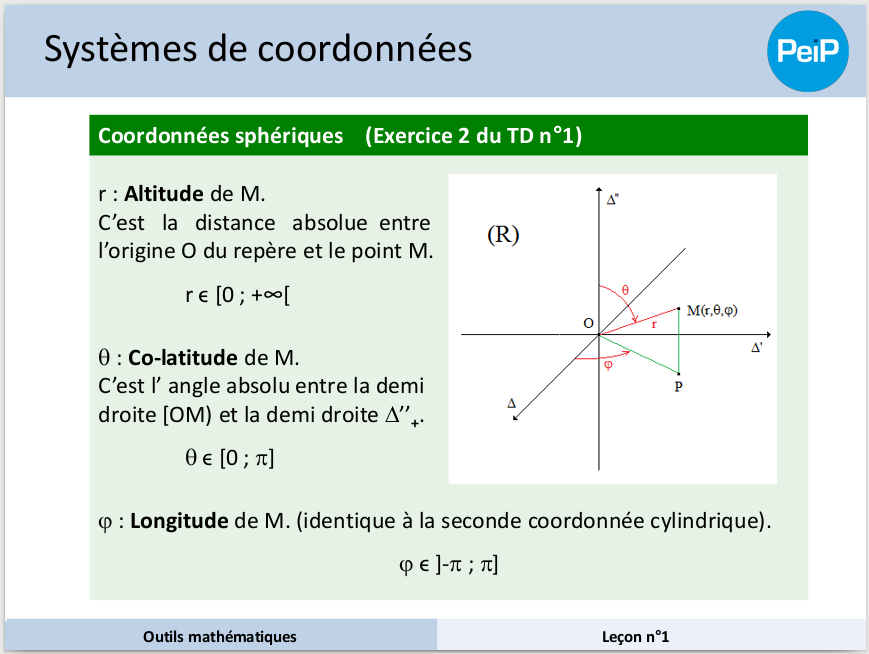
\includegraphics[width=.25\textwidth]{../figures/l1coordSpherique.png}%
        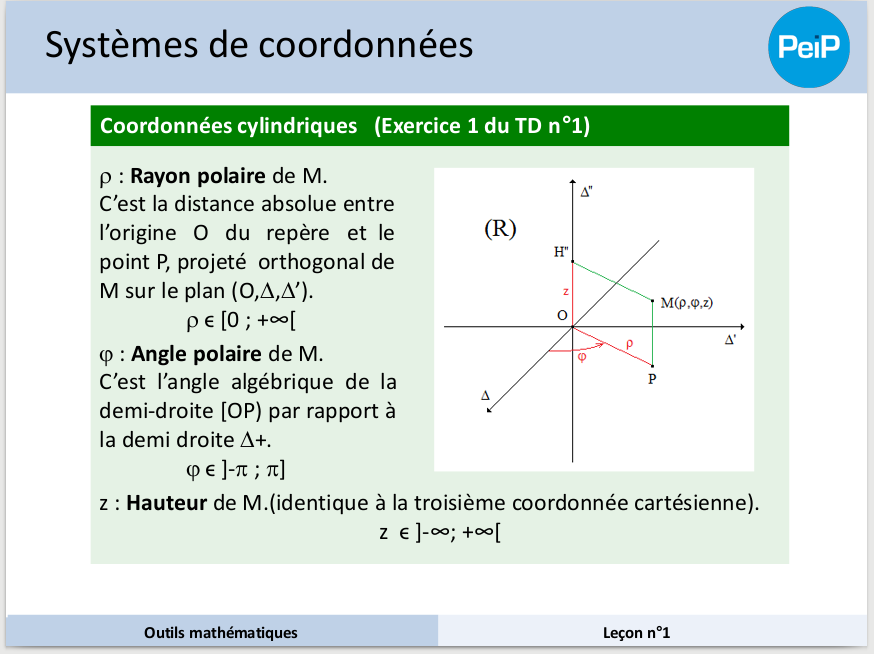
\includegraphics[width=.25\textwidth]{../figures/l1coordlcylindrique.png}%
        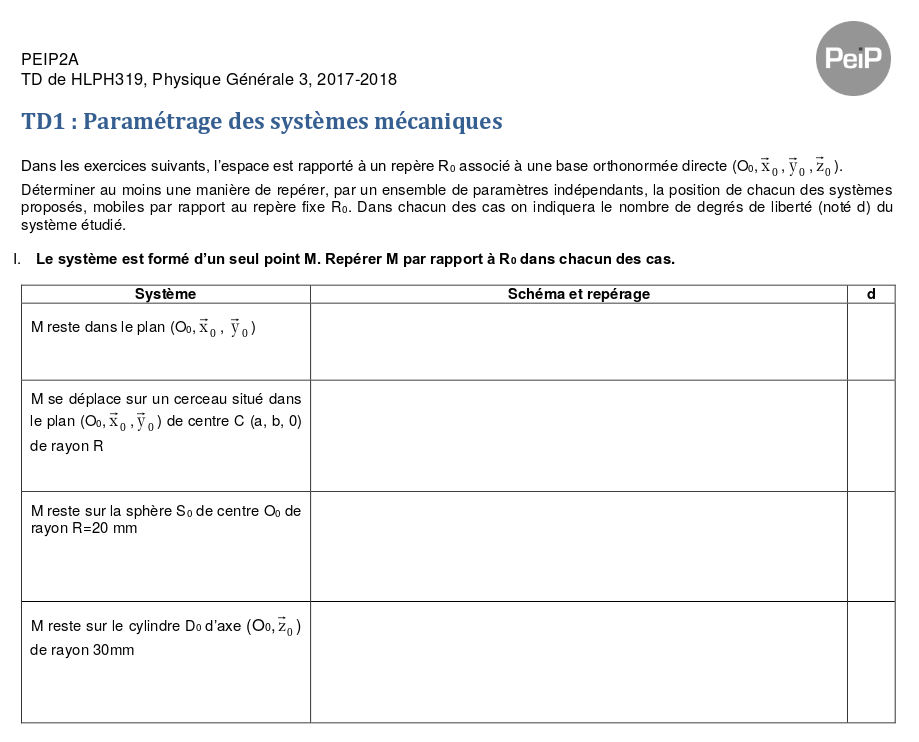
\includegraphics[width=.25\textwidth]{../figures/td1mecanique.png}
    \end{center}
}

\sld{\vfill\pagebreak[5]}%%%%%%%%%%%%%%%

\section{Espaces affines}

\subsection{Points et vecteurs}

On modélise le plan et l'espace par des espaces affines de dimension 2 et 3 respectivement. Pour l'espace à 3 dimensions on considère l'ensemble $\R^3$ des triplets de réels:
\begin{enumerate}
	\item Ensemble $\mathcal E$ des points: On peut décrire un point $M$ de l'espace (\ie une \emph{position}) par un triplet $(x,y,z)\in\R^3$ de réels. 

\sld{\vfill\pagebreak[5]}%%%%%%%%%%%%%%%

	\item Ensemble $E$ de vecteurs:  on peut aussi voir $E=\R^3$ comme un espace vectoriel. Un vecteur $u\in E$ modélise alors un ``\emph{déplacement}'' entre 2 points $A$ et $B$ de $\Ee$. Si $A = (a_1,a_2,a_3)$ et $B=(b_1,b_2,b_3)$ on définit le vecteur $u = \overrightarrow{AB}$ comme étant le triplet de réels $u = (b_1-a_1,b_2-a_2,b_3-a_3)$. %On note généralement $u= \overrightarrow{AB}$.
%Les règles de calculs usuelles 
On a alors: 
		\begin{enumerate}
			\item Pour tout $u \in E$ et $(A,B) \in \Ee$: $u +A = \overrightarrow{AB} + A = B \in \Ee$
				\sld{\begin{center}
						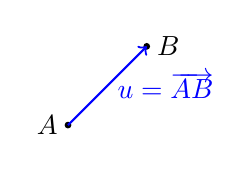
\begin{tikzpicture}
							\coordinate (a) at (0,0)  ;
							\coordinate (b) at (1,1) ;
							\filldraw[black] (a) circle (1pt);
							\filldraw[black] (b) circle (1pt);
							\draw[->, thick,blue] (a) node[left,black] {$A$} --  node[right, blue] {$u = \overrightarrow{AB}$}(b) node[right,black] {$B$};
						\end{tikzpicture}
					\end{center}
				}\pl{\rep{3cm}\pagebreak[4]}
\sld{\vfill\pagebreak[5]}%%%%%%%%%%%%%%%
			\item Relation de Chasles: $\forall A,B,C \in \Ee$ on a $\overrightarrow{AB} + \overrightarrow{BC} = \overrightarrow{AC}$.
				\sld{
\begin{center}
	\begin{tabular}{cc}
		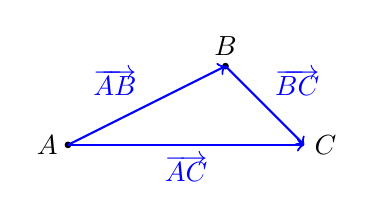
\begin{tikzpicture}
			\coordinate (a) at (0,0)  ;
			\coordinate (b) at (2,1) ;
			\coordinate (c) at (3,0) ;
			\filldraw[black] (a) circle (1pt);
			\filldraw[black] (b) circle (1pt);
			\draw[->, thick,blue] (a) node[left,black] {$A$} --  node[ above left, blue] {$\overrightarrow{AB}$}(b) node[above,black] {$B$};
			\draw[->, thick,blue] (b) --  node[above right, blue] {$\overrightarrow{BC}$}(c) node[right,black] {$C$};
			\draw[->, thick,blue] (a) --  node[below, blue] {$\overrightarrow{AC}$}(c);
		\end{tikzpicture} 
		&
		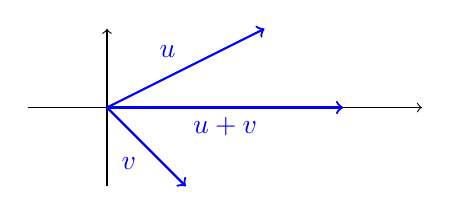
\begin{tikzpicture}
			\coordinate (a) at (0,0)  ;
			\coordinate (b) at (2,1) ;
			\coordinate (c) at (3,0) ;
			\draw[->] (0,-1) -- (0,1) ;
			\draw[->] (-1,0) -- (4,0) ;
			\draw[->, thick,blue] (a) --  node[ above left, blue] {$u$}(b);
			\draw[->, thick,blue] (a) --  node[below left, blue] {$v$}( 1,-1);
			\draw[->, thick,blue] (a) --  node[below, blue] {$u+v$}(c);
		\end{tikzpicture}
		\\
		dans $\Ee$ & dans $E$
	\end{tabular} 
\end{center}
} 

\pl{\rep{4cm}}
	\end{enumerate}
\end{enumerate}
En résumé, les éléments de $\Ee$ sont considérés comme des points (notés en majuscules) sur lesquels opèrent des vecteurs (notés en minuscules) de $E$. 

%La relation entre couples de points  et vecteurs est précisée dans la définition suivante~:%On peut axiomatiser la construction des espaces affines avec la définition suivante:
%\begin{definition}
%	Soit $E$ un \rev{}. Un espace affine dirigé par $E$ est un ensemble $\mathcal E$ non vide, muni d'une application $\varphi: \mathcal E \times \mathcal E \to E$ vérifiant les axiomes suivants:
%	\begin{enumerate}
%		\item pour tout $A,B,C\in \mathcal E$ on a $\varphi(A,C) = \varphi(A,B) +  \varphi(B,C)$ (\emph{relation de Chasles}),
%		\item pour tout $A \in \mathcal E$ et pour tout $x\in E$, il existe un unique $B \in \mathcal E$ tel que $x = \varphi(A,B)$ (\ie l'application $\varphi_A:M\mapsto\varphi(A,M)$ est une bijection de $\mathcal E$ dans $E$).
%	\end{enumerate}
%\end{definition}
%\begin{remark}
%	Dans le cas de l'espace, un couple de points $(A,B) \in \Ee^2$ est appelé un \emph{bipoint} auquel on associe le vecteur $\varphi(A,B) \in \R^3$ qui est noté $\overrightarrow{AB}$.
%\end{remark}

\sld{\vfill\pagebreak[5]}%%%%%%%%%%%%%%%
\subsection{Repère de l'espace} 

%\subsubsection{définitions}

\begin{definition}[(Repère cartésien)]
Un repère cartésien de l'espace $\Ee$ est la donnée d'un point $\Omega$ (l'origine du repère) et de trois vecteurs $(e_1,e_2,e_3)$ formant une base (\ie une famille libre g\'en\'eratrice) de l'espace $E$.
\end{definition}
\pl{\rep{3cm}}
\begin{definition}[(coordonnées cartésiennes)]
	Si $M$ est un point de $\Ee$ alors le vecteur $\overrightarrow{\Omega M}$ se décompose de façon unique sur les vecteurs de base:
	\[
		\overrightarrow{\Omega M} = x_1 e_1 + x_2 e_2 + x_3 e_3 
	\]
	Le triplet $\begin{psmallmatrix}x_1 \\ x_2 \\ x_3\end{psmallmatrix}_{\mathcal R}$ (ou plus simplement $\begin{psmallmatrix}x_1\\x_2\\ x_3\end{psmallmatrix}$ si il n'y a pas d'ambiguïtés) contient les coordonnées cartésiennes du point $M$ dans le repère $\mathcal R$.
\end{definition}
\pl{\rep{3cm}}

\sld{\vfill\pagebreak[5]}%%%%%%%%%%%%%%%
\begin{remark}
	Une fois une origine $\Omega$ de repère choisie, on peut identifier un point $M$ de $\Ee$ avec le vecteur $\overrightarrow{\Omega M} \in E$. 
	Alors, le choix d'un syst\`eme de coordonn\'ees permet de ramener tous les calculs \`a des calculs dans $\mathbb R^3.$
	Lorsque l'on ne précise pas la base, c'est que l'on se place dans l'espace vectoriel $E = \R^3$ muni de la base canonique composée des vecteurs $i = \begin{psmallmatrix}1\\0\\0\end{psmallmatrix}$, $j=\begin{psmallmatrix}0\\1\\0\end{psmallmatrix}$ et $k=\begin{psmallmatrix}0\\0\\1\end{psmallmatrix}$. 
\end{remark}

\sld{\vfill\pagebreak[5]}%%%%%%%%%%%%%%%


\bigskip

\begin{remark}{\bf\sffamily Changement de repère:} \label{rem_cdr} Soit deux repères cartésiens $\mathcal R =(\Omega,e_1,e_2,e_3) $ et $\mathcal R' =(\Omega',e_1',e_2',e_3') $ et un point $M$. On note:
\begin{itemize}
	\item $\begin{psmallmatrix}x\\ y \\z \end{psmallmatrix}_{\mathcal R}$ les coordonnées de $M$ dans $\mathcal R$ et $\begin{psmallmatrix}x'\\y'\\z' \end{psmallmatrix}_{\mathcal R'}$ les coordonnées de $M$ dans $\mathcal R'$
	\item $\begin{psmallmatrix}\alpha\\\beta\\\gamma \end{psmallmatrix}_{\mathcal R}$ les coordonnées de $\Omega'$ dans la $\mathcal R$.
	\item $\begin{psmallmatrix} a_{1,i}\\a_{2,i}\\a_{3,i} \end{psmallmatrix}_{\mathcal R}$ les coordonnées des $e_i'$ (pour $i=1,2,3$) dans $\mathcal R$.
\end{itemize}
%Pour passer d'un reprère à l'autre on a la formule suivante: 
Alors les coordonnées du point $M$ dans le repère $\mathcal R$ s'expriment en fonction des coordonnées de $M$ dans le repère $\mathcal R$:
\[
	\begin{cases}
		x = \alpha +a_{1,1}x'+ a_{1,2}y' +a_{1,3} z'\\
		y = \beta  +a_{2,1}x'+ a_{2,2}y' +a_{2,3} z'\\
		z = \gamma +a_{3,1}x'+ a_{3,2}y' +a_{3,3} z'
	\end{cases} \Leftrightarrow \begin{pmatrix}
		x\\y\\y
	\end{pmatrix}_{\mathcal R}=\begin{pmatrix}
		\alpha\\\beta\\\gamma
	\end{pmatrix}_{\mathcal R}+ \begin{pmatrix}
		a_{1,1} & a_{1,2} & a_{1,3}\\
		a_{2,1} & a_{2,2}& a_{2,3} \\
		a_{3,1} & a_{3,2} & a_{3,3}
	\end{pmatrix}_{\mathcal R \leftarrow \mathcal R'} \begin{pmatrix}
		x'\\y'\\z'
	\end{pmatrix}_{\mathcal R'}.
\]
\end{remark}

\sld{\vfill\pagebreak[5]}%%%%%%%%%%%%%%%


\begin{remark}
A propos des notations: un élément de $\R^n$ sera noté par convention $(x_1,\cdots, x_n)$ (c'est la donnée de $n$ réels). Lorsque l'on note $\begin{pmatrix}x_1 & \cdots & x_n\end{pmatrix}$  (resp. $\begin{psmallmatrix}x_1 \\ \vdots \\ x_n\end{psmallmatrix}$) on manipule en fait une matrice ligne (resp. colonne) dont les entrées sont les coordonnées d'un élément $(\tilde x_1, \cdots, \tilde x_n)$ dans une base donnée (ainsi lorsque les virgules disparaissent il y eut choix de base...). En général, les matrices colonnes représentent des vecteurs et les matrices lignes des formes linéaires (des fonctions linéaires à valeurs réelles).
\end{remark}
\sld{\vfill\pagebreak[5]}%%%%%%%%%%%%%%%
\subsection{Droites et plans affines}

\begin{definition}% [(Droite vectorielle, droite affine)]
Soit $\Ee$ un espace affine dirigé par un espace vectoriel $E$: 
	\begin{enumerate}
		\item Dans $E$: la \emph{droite vectorielle} engendrée par un vecteur $u\in E$ non-nul est l'ensemble des vecteurs colinéaires à $u$:
			\[
\redspace
				\vect(u) = \left\{ v\in E, \exists \lambda \in \R, v = \lambda u \right\} = \R u.
			\]
\pl{\rep{3cm}}
Si deux vecteurs $(u,v) \in E^2$ sont non-colinéaires, le \emph{plan vectoriel} engendré par $(u,v)$ est l'ensemble des vecteurs combinaisons linéaires de $u$ et $v$:
			\[
\redspace
				\vect(u,v) = \left\{ w\in E, \exists \lambda,\mu \in \R, w = \lambda u + \mu v \right\}.
			\]
\pl{\rep{3cm}}
		\item	Dans $\mathcal E$: la \emph{droite affine} $\mathcal D$ passant par un point $A$ et dirigée par un vecteur non-nul $u\in E$ est l'ensemble des points 
			\[
\redspace
			\mathcal D = \left\{D\in\Ee\  | \  D = A + \lambda u, \lambda \in \R \right\} \subset \Ee.
		\]
		On note $\mathcal D = A + \vect (u)$ et on dit que $\vect(u)$ est la direction de $\mathcal D$. De même, le \emph{plan affine} $\mathcal P$ dirigé par $u,v$ est 
		\[
\redspace
			\mathcal P =\left\{ A  + (\lambda u + \mu v), \lambda,\mu \in \R \right\} = A + \vect(u,v) \subset \Ee.
		\]
\pl{\rep{3cm}}
	\end{enumerate}
\end{definition}

\sld{\vfill\pagebreak[5]}%%%%%%%%%%%%%%%



%\pl{\pagebreak[5]}

\section{Calcul vectoriel}

\subsection{Produit scalaire}

\begin{definition}
	Soit $u =(u_1,u_2,u_3)$ et $v=(v_1,v_2,v_3)$ deux vecteurs de $\R^3$. Le produit scalaire de $u$ et $v$ est
	\[
		\prs{u,v} = u_1v_1 + u_2v_2 + u_3v_3.
	\]
et on définit la \emph{norme} d'un vecteur $u=(u_1,u_2,u_3)$ par
\[
	\norm{u}^2  = {u_1^2+u_2^2+u_3^2}.
\]
\end{definition}
\begin{remark}
    Le produit scalaire et la norme (au carrée) sont donc des relations polynômiales homogènes (de degré 2) des coordonnées de $u$ et $v$.
\end{remark}

\sld{\vfill\pagebreak[5]}%%%%%%%%%%%%%%%

\noindent{\bf\sffamily  Interprétation géométrique:} Soit $u$ et $v$ deux vecteurs  de $\R^3$ dont la norme est égale à 1:
\sld{
	\begin{center}
	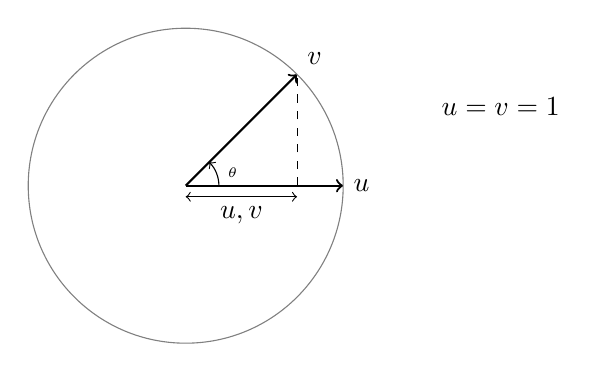
\begin{tikzpicture}[scale=2]
		\draw[->,thick] (0,0) -- (1,0) node [right] {$u$};
		\draw[->,thick] (0,0) -- (0.707106781,0.707106781) node [above right] {$v$};
		\draw[thin, gray] (0,0) circle (1);
		\draw[dashed] (0.707106781,0) -- (0.707106781,0.707106781);
		\draw[](0,0) -- (0.707106781,0); 
		\draw[<->,thin](0,-2pt) -- node[below]{$\prs{u,v}$}(0.707106781,-2pt); 
		\draw[->] (6pt,0) arc (0:45:6pt) node[midway, right=.5pt] {\tiny  $\theta$};
		\node at (2.0,.5) {$\snorm{u} = \snorm{v} =1$};
	\end{tikzpicture}
\end{center}
} \pl{\rep{4cm}}
Le produit scalaire de deux vecteurs unitaires est donc le cosinus de l'angle $\theta$ entre les vecteurs.
De plus, on a la formule suivante pour tout $u,v\in\R^3$:
\[
	\prs{u,v} = \norm{u}\norm{v} \cos(\theta).
\]
%et la propriété suivante (admise pour l'instant) 
%\[
	%\prs{u,v} \leq \norm{u}\norm{v}
%\]
En découle la majoration suivante \[\abs{\prs{u,v}} \leq \snorm{u}\snorm{v}\] avec cas d'égalité si $u$ et $v$ sont colinéaires.

%{\bf Interprétation en terme de projection ?}
%{\bf formule du cos de l'angle en fonction des coordonnée?}

\bigskip

\begin{proposition} Le produit scalaire satisfait aux règles de calculs suivantes:
	\begin{enumerate}
		\item \emph{Bilinéarité}: soient $u,v,w \in \R^3$ et $\lambda,\mu\in \R$:
			\begin{enumerate}
				\item  $\prs{\lambda u + \mu v, w} = \lambda \prs{u,w} + \mu \prs{v,w} $
				\item $\prs{u,\lambda v + \mu w} = \lambda \prs{u,v} + \mu \prs{u,w} $ 
			\end{enumerate}
		\item \emph{Symétrie}: soient $u,v\in\R^3$ $\prs{u,v} = \prs{v,u}$.
	\end{enumerate}
\end{proposition}

\begin{proof}
\pl{\rep{5cm}}	
\end{proof}

\sld{\vfill\pagebreak[5]}%%%%%%%%%%%%%%%

\begin{definition}
	\begin{enumerate}
		\item On dit que deux vecteurs sont \emph{orthogonaux} lorsque leur produit scalaire est nul.
		\item On dit qu'un vecteur est \emph{unitaire} lorsque sa norme vaut 1.
		\item On dit qu'une base est \emph{orthonormale} lorsque les trois vecteurs de la base sont orthogonaux deux à deux et unitaires. On utilise l'acronyme ``B.O.N.'' pour base orthonormale.
		\item On dit qu'un repère est \emph{orthonormé} lorsque sa base est orthonormale.
	\end{enumerate}
\end{definition}


%\subsubsection{Changement de base}

\begin{proposition}[(coordonnées d'un vecteur dans une B.O.N.)]
	Dans une base orthonormale $(e_1,e_2,e_3)$ de $\R^3$, un vecteur $u\in\R^3$ se décompose sous la forme\[
		u = \prs{e_1,u} e_1 + \prs{e_2,u} e_2 + \prs{e_3,u} e_3
	\]
\end{proposition}

\begin{proof}
\pl{\rep{4cm}}		
\end{proof}

\sld{\vfill\pagebreak[5]}%%%%%%%%%%%%%%%

\begin{proposition}[(Calcul du produit scalaire dans une B.O.N.)]
Si $(e_1,e_2,e_3)$ est une base orthonormale quelconque de $\R^3$ et si  $u = x_1 e_1 + x_2 e_2 + x_3 e_3$ et $v = y_1 e_1 + y_2 e_2 + y_3 e_3$ sont deux vecteurs de $\R^3$, alors le produit scalaire de $u$ et $v$ s'écrit:
\[
\prs{u,v} = x_1 y_1 + x_2y_2 + x_3y_3. 
\]
\end{proposition}

\begin{proof}
\pl{\rep{4cm}}		
\end{proof}

\sld{\vfill\pagebreak[5]}%%%%%%%%%%%%%%%

\begin{definition}
	On définit la \emph{distance} entre deux points $A$ et $B$ de l'espace $\Ee$ par:
	\[
		d(A,B) = \snorm{\overrightarrow{AB}}
	\]
	Si $\mathcal R$ est un repère orthonormé on a 
	\[
		d(A,B) = \sqrt{(x_1-y_1)^2+ (x_2-y_2)^2 + (x_3-y_3)^2 }
	\]
	où $\begin{psmallmatrix}
		x_1\\x_2\\x_3
	\end{psmallmatrix}_{}$ et $\begin{psmallmatrix}
		y_1\\y_2\\y_3
	\end{psmallmatrix}_{}$ sont les coordonnées dans $\mathcal R$ de $A$ et de $B$ respectivement.
\end{definition}

\sld{\vfill\pagebreak[5]}%%%%%%%%%%%%%%%
\section{Repérage}

\subsection{Orientation du plan et de l'espace}
Un repère orthonorm\'e $\mathcal R = \left(\Omega,e_1,e_2,e_3 \right)$ \'etant choisi, on rappelle que, pour exprimer les coordonn\'ees
d'un point dans un autre rep\`ere $\mathcal R' = \left(\Omega',e'_1,e'_2,e'_3 \right)$ il est n\'ecessaire d'utiliser la matrice de passage $B$
de la base $(e_1,e_2,e_3)$ \`a la base $(e'_1,e'_2,e'_3)$ (voir la {\bf Remarque \ref{rem_cdr}}). Si la nouvelle base est orthonom\'ee, on peut montrer que ${\rm det}(B) \in \{1,-1\}$ et a donc seulement deux valeurs possibles qui correspondent \`a deux orientations de l'espace. 

\begin{remark}
    D'un point de vue pratique, ceci s'illustre par le fait qu'un contorsionniste aussi dou\'e qu'il soit ne pourra pas superposer ses deux mains, droite et gauche.
\end{remark}

\sld{\vfill\pagebreak[5]}%%%%%%%%%%%%%%%

Il faut alors choisir une convention pour ``orienter l'espace'' et on se contente ici de décrire l'une des règles classiques  dite ``règle des 3 doigts de la main droite'' (il en existe d'autres comme la règle du ``bonhomme d'ampère'' ou la règle du ``tire bouchon'' qui suivent toutes la même convention): on dit qu'un repère est \emph{direct} si le pouce, l'index et le majeur de la main droite peuvent être placés (direction et sens) suivant les vecteurs $(e_1,e_2,e_3)$.
%On privilégiera bien sûr la représentation directe des axes $(Ox,Oy,Oz)$:

\begin{center}
	\begin{tabular}{c}
		\begin{tikzpicture}
			\def\side{2}
			%\draw[white,thick,->] (0,0,0) -- (0,0,\side+.3) node[below right,text width=1.4cm, align=center]{$z$ (majeur)} ;
			\draw[thick,->] (0,0,0) -- (\side+.3,0,0) node[right] {$x$};
			\draw[thick,->] (0,0,0) -- (0,\side+.3,0) node[above] {$y$};
			\draw[thick,->] (2,1) arc (0:90:1cm) node[above right,midway]{$+$};
		\end{tikzpicture}
	\\
		Repère direct du plan
	\end{tabular}
	\begin{tabular}{c}
		%\usetikzlibrary{3d}
\begin{tikzpicture}
	[%x={(-0.5cm,-0.5cm)},
%	    y={(1cm,0cm)},
%	    z={(0cm,1cm)}, 
		scale=1,
		fill opacity=1,%0.80,
		very thin,
	every node/.append style={transform shape}]

\def\ctr{1}
\def\side{2}
\def\sideT{.4}
\filldraw[color=blue!40] (-\sideT,-\sideT,0) -- (-\sideT,\side,0) -- (\side,\side,0) -- (\side,-\sideT,0) -- cycle;
\filldraw[color=gray!40] (-\sideT,0,-\sideT) -- (-\sideT,0,\side) -- (\side,0,\side) -- (\side,0,-\sideT) -- cycle;
\filldraw[color=green!40] (0,-\sideT,-\sideT) -- (0,-\sideT,\side) -- (0,\side,\side) -- (0,\side,-\sideT) -- cycle;

\def\sideT{0}
\filldraw[color=blue!40] (-\sideT,-\sideT,0) -- (-\sideT,\side,0) -- (\side,\side,0) -- (\side,-\sideT,0) -- cycle;
\filldraw[color=gray!40] (-\sideT,0,-\sideT) -- (-\sideT,0,\side) -- (\side,0,\side) -- (\side,0,-\sideT) -- cycle;
	\filldraw[color=green!40] (0,-\sideT,-\sideT) -- (0,-\sideT,\side) -- (0,\side,\side) -- (0,\side,-\sideT) -- cycle;

%	% face #3
	\begin{scope}[canvas is zx plane at y=0]
		\draw[thick,->] (1.5,1) arc (0:90:.5cm) node[above right,midway]{$+$};
		\node[rotate=90] at (\ctr/2,\ctr) {plan $xz$};
	\end{scope}
%	% face #2
	\begin{scope}[canvas is yx plane at z=0]
		\draw[thick,<-] (1.5,1) arc (0:90:.5cm) node[above right,midway]{$+$};
		\node[yscale=-1,rotate=-90] at (\ctr/2,\ctr) {plan $xy$};
	\end{scope} 
%
%      % face #1
	\begin{scope}[canvas is yz plane at x=0]
		\draw[thick,->] (1.5,1) arc (0:90:.5cm) node[above right,midway]{$+$};
		\node[rotate=-90] at (\ctr/2,\ctr) {plan $yz$};
	\end{scope}

	\draw[thick,->] (0,0,0) -- (\side+.3,0,0) node[right,text width=2cm, align=center] {$x$ (pouce)};
	\draw[thick,->] (0,0,0) -- (0,\side+.3,0) node[above,text width=2.1cm, align=center] {$y$ (index)};
	\draw[thick,->] (0,0,0) -- (0,0,\side+.3) node[below left,text width=2.4cm, align=center] {$z$ (majeur)};

\end{tikzpicture}
 
		% version with pst-figure3d
%\psset{viewpoint=50 20 30 rtp2xyz,Decran=50}
%\begin{pspicture}[solidmemory](-4,-4)(6,5)
%%\psset{unit=0.5}

%\psSolid[object=plan,action=draw,definition=equation,args={[0 0 1 0]}, base=-4 4 -4 4,fillcolor=black!15,fillstyle=solid,name=P0]
%\psProjection[object=texte,fontsize=100,linecolor=red,text=slice,phi=90,plan=P0]

%%\psSolid[object=cube,a=8,action=draw,name=A,linecolor=red]

%%\psSolid[object=plan,action=none,definition=solidface,args=A 4,name=P1]
%%\psProjection[object=texte,fontsize=50,text=lateral,phi=-90,plan=P1](-5,0)

%\psSolid[object=plan,action=draw,definition=equation,args={[0 1 0 0]},opacity=.2, base=-4 4 -4 4,fillcolor=black!15,name=P2]
%%\psProjection[object=texte,fontsize=50,text=axial,phi=90,plan=P2](0,7)
%%\psSolid[object=plan,action=none,definition=equation,args={[1 0 0 0]},name=P3]
%%\psProjection[object=texte,action=draw,fontsize=50,text=temporal,phi=90,plan=P3](4,8)
%\axesIIID(0,0,0)(4,4,4)
%\end{pspicture}

%\psset{unit=0.45}
%\psset{viewpoint=50 40 30 rtp2xyz,Decran=50}
%\psset{lightsrc=viewpoint}
%\begin{pspicture}(-7,-8)(7,8)
%\psSurface[ngrid=.25 .25](-4,-4)(4,4){((y^2)-(x^2))/4 }
%\end{pspicture}

%\psset{viewpoint=30 40 20 rtp2xyz,Decran=30}
  %\begin{pspicture}(-3.5,-3.5)(3.5,3.5)
%%  \axesIIID(2,2,2)(4,4,4)
   %\psSolid[object=cube,a=4,fillcolor=blue,opacity=0.2,action=draw*]%
   %\psSolid[object=sphere,r=1.5,linewidth=0.1pt,ngrid=20 20,fillcolor=red,opacity=0.2,action=draw*]%
   %\psSolid[object=vecteur,args=0 -2 0](2,2,-2)
   %\psSolid[object=vecteur,args=-2 0 0](2,2,-2)
   %\psSolid[object=vecteur,args=0 0 2](2,2,-2)
   %\psPoint(2,2,0.2){Z}\rput(Z){z}\psPoint(2,-0.2,-2){X}\rput(X){x}\psPoint(-0.2,2,-2){Y}\rput(Y){y}
   %\psPoint(2,-1.6,-2){a1}\psPoint(2,-1.6,2){a2}\pcline{<->}(a1)(a2)\ncput*{d}
   %\psPoint(2,-1.6,2){a1}\psPoint(-2,-1.6,2){a2}\pcline{<->}(a1)(a2)\ncput*{d}
   %\psPoint(-1.6,2,-2){a1}\psPoint(-1.6,2,2){a2}\pcline{<->}(a1)(a2)\ncput*{d}
   %\psPoint(0,0,0){a1}\psPoint(1,-1,0){a2}\pcline{->}(a1)(a2)\ncput*{r}
  %\end{pspicture}

%\begin{tikzpicture}
%\def\zlength{-0.5cm}
%\foreach \zangle [count=\i from 0] in {10,30,...,80}{
%\begin{scope}[shift={({mod(\i,2)*4cm},{-floor(\i/2)*4cm})}, 
    %x=(0:1cm), y=(90:1cm),z=(\zangle:\zlength)]
%%\def\zangle{80}
    %\def\sliceZ{0}
    %\def\side{2}
    %% draw plane
    %\filldraw[color=gray!40] (0,0,0) -- (0,0,\side) -- (\side,0,\side) -- (\side,0,0) -- cycle;
    %\filldraw[color=gray!40] (0,0,0) -- (0,\side,0) -- (\side,\side,0) -- (\side,0,0) -- cycle;
    %\filldraw[color=gray!40] (0,0,0) -- (0,0,\side) -- (,0\side,\side) -- (0,\side,0) -- cycle;
     %%\draw[dashed] (0,\sliceZ,0) -- (0,\sliceZ,\side) -- (\side,\sliceZ,\side) -- (\side,\sliceZ,0) -- cycle;
    %% draw axes
    %\draw[->] (0,0,0) -- (\side+.3,0,0) node[right] {$x$};
    %\draw[->] (0,0,0) -- (0,\side+.3,0) node[below] {$y$};
    %\draw[->] (0,0,0) -- (0,0,\side+.3) node[below] {$z$};
    %\node[cm={1,0,cos(\zangle),sin(\zangle),(0,0)}] at (1,1,0){plan $x-y$};
    %\node[cm={1,0,cos(\zangle),sin(\zangle),(0,0)}] at (1,0,1){plan $x-z$};
    %\node[cm={1,0,cos(\zangle),sin(\zangle),(0,0)}] at (0,1,1){plan $x-z$};
%\end{scope}
%}
%\end{tikzpicture}
\begin{tikzpicture}
    [%x={(-0.5cm,-0.5cm)},
%	    y={(1cm,0cm)},
%	    z={(0cm,1cm)}, 
    scale=1,
    fill opacity=1,%0.80,
    very thin,
    every node/.append style={transform shape}]
\newcommand\drawface{\draw[fill=gray!100] (-.2,-.2) rectangle (2,2)}

\def\ctr{1}
\def\side{2}
\def\sideT{.4}
\filldraw[color=green!40] (-\sideT,-\sideT,0) -- (-\sideT,\side,0) -- (\side,\side,0) -- (\side,-\sideT,0) -- cycle;
\filldraw[color=blue!40] (-\sideT,0,-\sideT) -- (-\sideT,0,\side) -- (\side,0,\side) -- (\side,0,-\sideT) -- cycle;
\filldraw[color=gray!40] (0,-\sideT,-\sideT) -- (0,-\sideT,\side) -- (0,\side,\side) -- (0,\side,-\sideT) -- cycle;

\def\sideT{0}
\filldraw[color=green!40] (-\sideT,-\sideT,0) -- (-\sideT,\side,0) -- (\side,\side,0) -- (\side,-\sideT,0) -- cycle;
\filldraw[color=blue!40] (-\sideT,0,-\sideT) -- (-\sideT,0,\side) -- (\side,0,\side) -- (\side,0,-\sideT) -- cycle;
\filldraw[color=gray!40] (0,-\sideT,-\sideT) -- (0,-\sideT,\side) -- (0,\side,\side) -- (0,\side,-\sideT) -- cycle;
	% face #3
	\begin{scope}[canvas is zx plane at y=0]
	   %\drawface;
		\draw[thick,->] (1.5,1) arc (0:90:.5cm) node[above right,midway]{$+$};
	   \node[rotate=90] at (\ctr/2,\ctr) {plan $xy$};
	\end{scope}
	% face #2
	\begin{scope}[canvas is yx plane at z=0]
	   %\drawface;
		\draw[thick,<-] (1.5,1) arc (0:90:.5cm) node[above right,midway]{$+$};
	   \node[yscale=-1,rotate=-90] at (\ctr/2,\ctr) {plan $yz$};
	\end{scope} 

       % face #1
	\begin{scope}[canvas is yz plane at x=0]
	    %\drawface;
		\draw[thick,->] (1.5,1) arc (0:90:.5cm) node[above right,midway]{$+$};
	    \node[rotate=-90] at (\ctr/2,\ctr) {plan $xz$};
	\end{scope}



	\draw[thick,->] (0,0,0) -- (\side+.3,0,0) node[right,text width=2.1cm, align=center] {$y$ (index)};
	\draw[thick,->] (0,0,0) -- (0,\side+.3,0) node[above,text width=2.4cm, align=center]{$z$ (majeur)} ;
	\draw[thick,->] (0,0,0) -- (0,0,\side+.3) node[below left,text width=2cm, align=center] {$x$ (pouce)};
\end{tikzpicture}

	\\
	Repères directs de l'espace
	\end{tabular}
\end{center}
Une permutation circulaire de trois vecteurs ne modifie pas son orientation et les deux repères ci-dessus sont directs. Si on change l'orientation d'un des vecteurs, on change l'orientation du repère (orientation \emph{indirecte}). Dans la suite de ce cours nous considèrerons toujours des repères directs.


\subsection{Coordonnées polaires}



Dans le plan muni d'un repère $(\Omega; e_1,e_2)$. Un point $M$ est décrit par une distance $r\in \R^+$ et un angle $\theta \in [0,2\pi[$. On a 
	\[\redspace
		\begin{cases}
			r^2 = x^2 + y^2\\
			\tan(\theta) = \frac{y}{x} 
		\end{cases} \Leftrightarrow \begin{cases}
			x = r\cos(\theta)\\
			y = r\sin(\theta)
		\end{cases}
	\]

	\begin{center}

	\pgfmathsetmacro{\sradius}{.2}
		\begin{tikzpicture}
			[scale=4,]

%draw the main coordinate system axes
		\draw[thick,->] (-.1,0) -- (.6,0) node[anchor=south]{$x$};
		\draw[thick,->] (0,-.1) -- (0,.6) node[anchor=north west]{$y$};


% (-z x y)

		\draw (.5, .5) node [circle,fill=red, inner sep=.02cm] () {};

		\draw[dashed,red] (.5, .5, 0) node[above right]{$M$}-- (.5,0,0);
		\draw[dashed,red] (.5, .5, 0) node[above]{}-- (0,.5,0);
		\draw[thick,red] (.5, .5, 0) -- node[midway,above left]{$r$} (0,0,0);

		\draw[thick,red] (0, 0, 0) -- (.5, .5,0);

		\draw[thick,->,red] (\sradius,0) arc (0:45:\sradius)node[midway,right]{$\theta$}  ;

		\end{tikzpicture}
	\end{center}
Attention, en l'état, il n'y a pas unicité des coordonnées polaires pour l'origine.
\sld{\vfill\pagebreak[5]}%%%%%%%%%%%%%%%
\subsection{Coordonnées cylindrique}


Dans l'espace avec $(\Omega;e_1,e_2,e_3)$ un repère orthonormé direct. On décrit la position d'un point $M$ par un triplet (distance, angle, hauteur)$=(r,\theta,z) \in \R^+ \times [0, 2\pi[ \times \R$. On a
\sld{\vfill\pagebreak[5]}%%%%%%%%%%%%%%%
\[
	\begin{cases}
		x = r\cos(\theta)\\
		y= r\sin(\theta) \\
		z=z
	\end{cases}
\Leftrightarrow
\begin{cases}
	r^2 = x^2 + y^2\\
	\tan(\theta) = \frac y x \\
	z=z
\end{cases}.
\]

\begin{center}
	\tdplotsetmaincoords{60}{110}

	\pgfmathsetmacro{\radius}{.707106781}
	\pgfmathsetmacro{\sradius}{.3}

%start tikz picture, and use the tdplot_main_coords style to implement the display 
%coordinate transformation provided by 3dplot
	\begin{tikzpicture}[scale=3,tdplot_main_coords,]

%draw the main coordinate system axes
		\draw[thick,->] (-.1,0,0) -- (.8,0,0) node[anchor=north east]{$x$};
		\draw[thick,->] (0,-.1,0) -- (0,.8,0) node[anchor=north west]{$y$};
		\draw[thick,->] (0,0,-.1) -- (0,0,.8) node[anchor=south]{$z$};


		%\draw[dashed] (\radius,0,\radius) arc (0:360:\radius);
		\draw[dashed] (\radius,0,0) arc (0:360:\radius);
% (-z x y)
%\draw (0, 1, 0) node [circle,fill=black, inner sep=.02cm] () {};
		\draw (0, 0, \radius) node [circle,fill=black, inner sep=.02cm] () {};
%\draw (1, 0, 0) node [circle,fill=black, inner sep=.02cm] () {};

		\draw (.5, .5, .6) node [circle,fill=red, inner sep=.02cm] () {};

                \draw[thick,red] (.5, .5, .6) node[above right]{$M$}--node[pos=.3, right]{$z$} (.5,.5,0);
		\draw[dashed,red] (.5, .5, .6) -- (0,0,0.6);
		\draw[dashed,red] (.5, .5, 0) node[above]{}-- (.5,0,0);
		\draw[dashed,red] (.5, .5, 0) node[above]{}-- (0,.5,0);
		\draw[thick,red] (.5, .5, 0) -- node[midway,right]{$r$} (0,0,0);
		\draw[dashed,red] (0, 0, 0) -- (.5, .5, .6);
		\draw[thick,->,red] (\sradius,0,0) arc (0:45:\sradius)node[midway,below]{$\theta$}  ;

		\fill[top color=blue!10!white,bottom color=blue!10!white,middle color=blue!10!white,shading=axis,opacity=0.1](\radius,0,0) arc (0:360:\radius);
%\fill[left color=gray!50!black,right color=gray!50!black,middle color=gray!50,shading=axis,opacity=0.25] (0,-\radius,0,0) arc (0:180:\radius) -- (.707106781,0,.707106781) arc (90:-90:\radius) -- (0-\radius,\radius) arc (180:360:\radius);
%\draw[->,blue] (0,-\radius,0) arc (-90:90:\radius) -- (0,.707106781,.707106781) arc (90:-90:\radius) -- (0,-\radius,0) -- cycle;

	%	\fill[top color=gray!90!,bottom color=gray!2,middle color=gray!30,shading=axis,opacity=0.1] (\radius,0,\radius) arc (0:360:\radius);

	\end{tikzpicture}
\end{center}


Attention, en l'état, il n'y a pas unicité des coordonnées cylindriques sur l'axe $Oz$.
\sld{\vfill\pagebreak[5]}%%%%%%%%%%%%%%%
\subsection{Coordonnées sphériques}

On se place toujours dans l'espace $(\Omega;e_1,e_2,e_3)$ muni d'un repère  orthonormé direct. De multiples conventions de coordonnées sphériques sont utilisées dans la littérature: on en décrit 2 ci-dessous. Mais attention, suivant les auteurs ou le contexte, une même quantité peut être notée de plusieurs manières. Bref, il faut se méfier et regarder attentivement les définitions. En cas de doute: faire un dessin.

\subsubsection{La convention (rayon,colatitude,longitude)}

Utilisée en mathématiques et en physique, on décrit un point $M$ de l'espace par le triplet: 
\begin{enumerate}
\item Rayon: c'est la distance à l'origine. Notation: $r \in \R^+$
\item Colatitude: angle entre l'axe vertical $(Oz)$ et le vecteur $\overrightarrow{OM}$. Notation: $\varphi \in [0,\pi]$
\item Longitude: c'est l'angle entre l'axe $(Ox)$ et le segment $\overrightarrow{OM'}$ où $M'$ est le projeté de $M$ sur le plan équatorial. Notation: $\theta \in [0,2\pi[$.
\end{enumerate}
\[
	\begin{cases}
		x = r\sin(\varphi) \cos(\theta)\\
		y = r \sin(\varphi) \sin(\theta)\\
	        z = r \cos(\varphi)
	\end{cases}
\Leftrightarrow
\begin{cases}
	r^2 = x^2+y^2+z^2 \\
	\cos(\varphi) = \frac{z}{\sqrt{x^2+y^2+z^2} } \\
	\tan(\theta) = \frac y x
\end{cases}
\]

\begin{center}
	\tdplotsetmaincoords{60}{110}

%define polar coordinates for some vector
%TODO: look into using 3d spherical coordinate system
	\pgfmathsetmacro{\radius}{1}
	\pgfmathsetmacro{\sradius}{.3}
	\pgfmathsetmacro{\thetavec}{0}
	\pgfmathsetmacro{\phivec}{0}

%start tikz picture, and use the tdplot_main_coords style to implement the display 
%coordinate transformation provided by 3dplot
        \begin{tikzpicture}[scale=2.5,tdplot_main_coords]
            \pgfmathsetmacro{\coordphi}{45}
            \pgfmathsetmacro{\coordtheta}{60}
            \pgfmathsetmacro{\coordr}{\radius}
            \pgfmathsetmacro\coordx{cos(\coordtheta)*sin(\coordphi) * \coordr}
            \pgfmathsetmacro\coordy{sin(\coordtheta)*sin(\coordphi) * \coordr}
            \pgfmathsetmacro\coordz{cos(\coordphi) * \coordr}

%draw the main coordinate system axes
            \draw[thick,->] (-.1,0,0) -- (1.1,0,0) node[anchor=north east]{$x$};
            \draw[thick,->] (0,-.1,0) -- (0,1.1,0) node[anchor=north west]{$y$};
            \draw[thick,->] (0,0,-.1) -- (0,0,1.1) node[anchor=south]{$z$};

            \tdplotsetthetaplanecoords{\phivec}

%draw some dashed arcs, demonstrating direct arc drawing
            \draw[dashed,tdplot_rotated_coords] (\radius,0,0) arc (0:90:\radius);
            \draw[dashed,tdplot_rotated_coords] (\radius,0,0) arc (0:-90:\radius);

            \draw[dashed] (\radius,0,0) arc (0:360:\radius);
            \shade[ball color=blue!10!white,opacity=0.2] (1cm,0) arc (0:-180:1cm and 5mm) arc (180:0:1cm and 1cm);
            % Draw intersection axes and unit sphere
            \draw (0, 1, 0) node [circle,fill=black, inner sep=.02cm] () {};
            \draw (0, 0, 1) node [circle,fill=black, inner sep=.02cm] () {};
            \draw (1, 0, 0) node [circle,fill=black, inner sep=.02cm] () {};

            % Draw point M and related lines
            \draw (\coordx, \coordy, \coordz) node [circle,fill=red, inner sep=.02cm] () {};

            \draw[dashed,red] (\coordx, \coordy, 0)  -- (\coordx,\coordy,\coordz) node[above]{$M$};
            \draw[dashed,red] (\coordx, \coordy, 0)  -- (\coordx,0,0);
            \draw[dashed,red] (\coordx, \coordy, 0)  -- (0,\coordy,0);
            \draw[dashed,red] (\coordx, \coordy, 0)  -- (0,0,0);

            \draw[thick,red] (0, 0, 0) -- node[midway,below right]{$r$} (\coordx, \coordy, \coordz);

            % Draw angle theta
            \draw[thick,->,red] (\sradius,0,0) arc (0:\coordtheta:\sradius)node[midway,below]{$\theta$}  ;

            % Draw angle phi
            \tdplotsetthetaplanecoords{\coordtheta}
            \draw[thick,<-,red,tdplot_rotated_coords] (\coordphi:\sradius) arc (\coordphi:0:\sradius) node[midway,above]{$\varphi$};
        \end{tikzpicture}

\end{center}



Attention, en l'état, il n'y a pas unicité des coordonnées sphériques sur l'axe $Oz$.

\subsubsection{La convention (rayon,latitude,longitude)}

Voici une autre convention (avec une référence plus ``géographique'), on décrit un point $M$ de l'espace par le triplet (rayon,latitude,longitude)$=(r,\delta,\theta) \in \R^+ \times \Big[-\frac{\pi}{2}, \frac{\pi}{2} \Big] \times [0,2\pi[$. On a 
\sld{\vfill\pagebreak[5]}%%%%%%%%%%%%%%%
\[
	\begin{cases}
		x = r\cos(\delta) \cos(\theta)\\
		y = r \cos(\delta) \sin(\theta) \\
	        z = r \sin(\delta)
	\end{cases}
\Leftrightarrow
\begin{cases}
	r^2 = x^2+y^2+z^2 \\
	\sin(\delta) = \frac{z}{\sqrt{x^2+y^2+z^2} } \\
	\tan(\theta) = \frac y x
\end{cases}
\]
On remarque que l'on a $\delta = \frac\pi2 - \varphi$ donnant $\cos(\delta) = \sin{\varphi}$ et $\sin(\delta) = \cos{\varphi}$.
\begin{center}
	\tdplotsetmaincoords{60}{110}

%define polar coordinates for some vector
%TODO: look into using 3d spherical coordinate system
	\pgfmathsetmacro{\radius}{1}
	\pgfmathsetmacro{\sradius}{.3}
	\pgfmathsetmacro{\thetavec}{0}
	\pgfmathsetmacro{\phivec}{0}

%start tikz picture, and use the tdplot_main_coords style to implement the display 
%coordinate transformation provided by 3dplot
        \begin{tikzpicture}[scale=2.5,tdplot_main_coords]
            \pgfmathsetmacro{\coordphi}{45}
            \pgfmathsetmacro{\coordtheta}{60}
            \pgfmathsetmacro{\coordr}{\radius}
            \pgfmathsetmacro\coordx{cos(\coordtheta)*sin(\coordphi) * \coordr}
            \pgfmathsetmacro\coordy{sin(\coordtheta)*sin(\coordphi) * \coordr}
            \pgfmathsetmacro\coordz{cos(\coordphi) * \coordr}

%draw the main coordinate system axes
            \draw[thick,->] (-.1,0,0) -- (1.1,0,0) node[anchor=north east]{$x$};
            \draw[thick,->] (0,-.1,0) -- (0,1.1,0) node[anchor=north west]{$y$};
            \draw[thick,->] (0,0,-.1) -- (0,0,1.1) node[anchor=south]{$z$};

            \tdplotsetthetaplanecoords{\phivec}

%draw some dashed arcs, demonstrating direct arc drawing
            \draw[dashed,tdplot_rotated_coords] (\radius,0,0) arc (0:90:\radius);
            \draw[dashed,tdplot_rotated_coords] (\radius,0,0) arc (0:-90:\radius);

            \draw[dashed] (\radius,0,0) arc (0:360:\radius);
            \shade[ball color=blue!10!white,opacity=0.2] (1cm,0) arc (0:-180:1cm and 5mm) arc (180:0:1cm and 1cm);
            % Draw intersection axes and unit sphere
            \draw (0, 1, 0) node [circle,fill=black, inner sep=.02cm] () {};
            \draw (0, 0, 1) node [circle,fill=black, inner sep=.02cm] () {};
            \draw (1, 0, 0) node [circle,fill=black, inner sep=.02cm] () {};

            % Draw point M and related lines
            \draw (\coordx, \coordy, \coordz) node [circle,fill=red, inner sep=.02cm] () {};

            \draw[dashed,red] (\coordx, \coordy, 0)  -- (\coordx,\coordy,\coordz) node[above]{$M$};
            \draw[dashed,red] (\coordx, \coordy, 0)  -- (\coordx,0,0);
            \draw[dashed,red] (\coordx, \coordy, 0)  -- (0,\coordy,0);
            \draw[dashed,red] (\coordx, \coordy, 0)  -- (0,0,0);

            \draw[thick,red] (0, 0, 0) -- node[midway,above left]{$r$} (\coordx, \coordy, \coordz);

            % Draw angle theta
            \draw[thick,->,red] (\sradius,0,0) arc (0:\coordtheta:\sradius)node[midway,below]{$\theta$}  ;

            % Draw angle phi
            \tdplotsetthetaplanecoords{\coordtheta}
            \draw[thick,<-,red,tdplot_rotated_coords] (\coordphi:\sradius) arc (\coordphi:90:\sradius) node[midway,right]{$\delta$};
        \end{tikzpicture}

\end{center}



Attention, en l'état, il n'y a pas unicité des coordonnées sphériques sur l'axe $Oz$.
